\documentclass{emulateapj}
%\documentclass[12pt,preprint]{aastex}

\usepackage{graphicx}
\usepackage{svg}
\usepackage{float}
\usepackage{amsmath}
\usepackage{epsfig,floatflt}
\usepackage{hyperref}
\usepackage[toc, page]{appendix}
\usepackage{verbatim, amsmath, amsfonts, amssymb, amsthm}
\usepackage[utf8]{inputenc}
\usepackage{textcomp}
\usepackage{float}
\usepackage{xcolor}
\usepackage{color}
\usepackage{listings}
\usepackage{booktabs}
\usepackage{fancyhdr}
\usepackage[T1]{fontenc}
\usepackage{url}
\usepackage[export]{adjustbox}
\usepackage{calc}
%\usepackage{caption}
\usepackage{subfig}
\usepackage{color}
\definecolor{light}{rgb}{0.5, 0.5, 0.5}
\def\light#1{{\color{light}#1}}

%Fixes float position for figure*, such that placement operators can be used (or else just top of page)
\usepackage{dblfloatfix}

\usepackage{accents}
\newcommand{\dbtilde}[1]{\accentset{\approx}{#1}}
\newcommand{\vardbtilde}[1]{\tilde{\raisebox{0pt}[0.85\height]{$\tilde{#1}$}}}

\usepackage{lipsum}
\usepackage[para]{footmisc}


\definecolor{mygreen}{rgb}{0,0.6,0}
\definecolor{mygray}{rgb}{0.5,0.5,0.5}
\definecolor{mymauve}{rgb}{0.58,0,0.82}

\lstset{ %
	backgroundcolor=\color{white}\ttfamily\tiny,   % choose the background color; you must add \usepackage{color} or \usepackage{xcolor}; should come as last argument
	basicstyle=\tiny,        % the size of the fonts that are used for the code \footnotesize,
	breakatwhitespace=false,         % sets if automatic breaks should only happen at whitespace
	columns=fullflexible,    %no spaces between columns
	keepspaces=true,
	breaklines=true,                 % sets automatic line breaking
	breakatwhitespace=true,
	captionpos=b,                    % sets the caption-position to bottom
	commentstyle=\color{mygreen},    % comment style
	deletekeywords={...},            % if you want to delete keywords from the given language
	escapeinside={\%*}{*)},          % if you want to add LaTeX within your code
	extendedchars=true,              % lets you use non-ASCII characters; for 8-bits encodings only, does not work with UTF-8
	frame=single,	                   % adds a frame around the code
	keepspaces=true,                 % keeps spaces in text, useful for keeping indentation of code (possibly needs columns=flexible)
	keywordstyle=\color{blue},       % keyword style
	language=Python,                 % the language of the code
	morekeywords={*,...},           % if you want to add more keywords to the set
	%numbers=left,                    % where to put the line-numbers; possible values are (none, left, right)
	%numbersep=5pt,                   % how far the line-numbers are from the code
	%numberstyle=\tiny\color{mygray}, % the style that is used for the line-numbers
	rulecolor=\color{black},         % if not set, the frame-color may be changed on line-breaks within not-black text (e.g. comments (green here))
	showspaces=false,                % show spaces everywhere adding particular underscores; it overrides 'showstringspaces'
	showstringspaces=false,          % underline spaces within strings only
	showtabs=false,                  % show tabs within strings adding particular underscores
	stepnumber=1,                    % the step between two line-numbers. If it's 1, each line will be numbered
	stringstyle=\color{mymauve},     % string literal style
	tabsize=1,	                   % sets default tabsize to 2 spaces
	%title=\lstname                   % show the filename of files included with \lstinputlisting; also try caption instead of title
}

\begin{document}

\title{A stock market model - Using Monte Carlo methods to simulate financial transactions}

\author{Bruce Chappell and Markus Bjørklund}

\email{markus.bjorklund@astro.uio.no}

\altaffiltext{1}{Institute of Theoretical Astrophysics, University of
  Oslo, P.O.\ Box 1029 Blindern, N-0315 Oslo, Norway}

\begin{abstract}
In this paper, we apply different models for assessing the interactions between financial agents in a theoretical stock market, acquiring an equilibrium distribution through Monte Carlo simulation. The models presented are uninfluenced transactions and transactions with saving, wealth preference and common transaction history. We find that the simulations produce the predicted Gibbs distribution in the first model, and also agree with analytical or empirical predictions in the latter cases, with the two latter most models tracing a Pareto distribution very well at the tail end. 

\end{abstract}
\keywords{Monte Carlo methods --- Stock market --- Finance}

\section{Introduction}
\label{sec:introduction}
Modeling financial structures has long been of interest, not only for applications in finance and politics. The outcome of a set of financial rules can vary greatly depending on the rule set in place, and modeling the outcome of such conditions is essential in order to assess whether the rules allow for a fair and desirable outcome.

However, the application of Monte Carlo systems to such models is a relatively new approach. In this paper, we will present four models with increasing degree of complexity for transactions between financial agents. We will account for factors such as saving, wealth preferences, and common transaction history. We will look at the equilibrium distributions for these models, that is what wealth distribution they tend to.

In this paper we will describe the fundamental theory in the theory section, provide the methods and algorithms implemented in the methods section, present essential figures and data in the results section, in addition to discussing the aforementioned results. We provide a summary and closing thoughts in the discussion section.

NOTE: Due to the high number of figures and their size, these are all presented in the appendix.

\section{Theory}
\subsection{Simulating transactions between financial agents}
We assume $N$ financial agents, each with a wealth of $m_i$, $i\in [1,N]$. Furthermore, we assume all agents start with an equal initial wealth of $m_i = m_0$. We let all agents start transacting with each other until we reach an equilibrium situation, a most likely state.

\subsection{Uninfluenced transactions}
Initially, we let the agents interact freely, ensuring the wealth is conserved
\begin{equation}
    m_i + m_j = m_i' + m_j'
\end{equation}
Where $m_i'$ and $m_j'$ is their respective wealth after the transaction. We accomplish this by picking two random agents $i$ and $j$, with respective wealth $m_i$ and $m_j$. They pool their wealth and redistribute it randomly by a factor drawn from a uniform distribution, I.E.

\begin{equation}
m_1'=\epsilon(m_1+m_2)
\end{equation}
\begin{equation}
m_2'=(1-\epsilon)(m_1+m_2),
\end{equation}

where $\epsilon \in [0,1]$ is drawn from the uniform distribution. This provides the desired conservation of wealth, shown by

$$m_1'+m_2'=\epsilon(m_1+m_2)+(1-\epsilon)(m_1+m_2)=m_1+m_2$$.

This model has an analytical equilibrium state given by the Gibbs distribution

\begin{equation}
    w_m = \beta \mathrm{exp} \left(-\beta m\right),
\end{equation}
where 
\begin{equation}
    \beta = \frac{1}{\langle m \rangle} \quad , \quad \langle m \rangle = \sum_i \frac{m_i}{N} = m_0
\end{equation}

\subsection{Transactions with saving}
We introduce the option of saving money into the model. We denote the fraction of money saved by the parameter $\lambda$, such that 

\begin{align}
m_i'&=\lambda m_i+\epsilon(1-\lambda)(m_i+m_j) \\
m_j'&=\lambda m_j+(1-\epsilon)(1-\lambda)(m_i+m_j).
\end{align}

We simplify the notation by writing 

\begin{align}
    m_i' &= m_i + \delta m \\
    m_j' &= m_j - \delta m,
\end{align}

with
\begin{equation}
    \delta m = \left(1-\lambda \right)\left(\epsilon m_j - \left(1-\epsilon\right)m_i\right).
\end{equation}

Conservation of wealth is still in effect, as shown below
\begin{equation}
    m_i'+m_j'= m_i + \delta m + m_j - \delta m = m_i + m_j.
\end{equation}
Also for $\lambda = 0$, I.E. no saving, this model reduces back to the the previous one. This model also as an analytical expression for the equilibrium state. For a normalized wealth $\tilde{m} = \frac{m}{\langle m \rangle}$, which is what is implemented in our code, it is shown in \cite{paper1} that we have an analytical solution for the wealth distribution given as 

\begin{equation}
w_{\tilde{m}}=\frac{n^n}{\Gamma(n)}\tilde{m}^{n-1}e^{-n\tilde{m}}
\end{equation}
Where $n$ is given by
\begin{equation}
    n=1+\frac{3\lambda}{1-\lambda},
\end{equation}
and $\Gamma(n)$ is the gamma-function.

This shows that, analytically, the distribution should approach a power law at the high end tail.

\subsection{Transactions with saving and wealth preferences}
Next, we introduce constraints on the interaction probability between agents. Instead of letting agents interact randomly, we introduce a distribution for the probability of interaction between agents. The distribution is biased, such that agents with comparable wealth are more likely to interact, given by

\begin{equation}
p_{ij} \propto \left|m_i-m_j \right|^{-\alpha},
\end{equation}
and $\alpha > 0$ is a positive parameter. We introduce the probability as is, with the exception of working with the normalized wealth $\tilde{m} = \frac{m}{\langle m \rangle}$, such that our PDF becomes

\begin{equation}
p_{ij} = \left|\frac{m_i-m_j}{m_0} \right|^{-\alpha},
\end{equation}

\subsection{Transactions with saving, wealth preferences and common transaction history}
Finally, we enhance the probability of interaction between agents, taking into account common transaction history. The likelihood of agents interacting will increase with the number of previous interactions, I.E.

\begin{equation}
p_{ij} \propto \left|m_i-m_j \right|^{-\alpha} \left(c_{ij} + 1\right)^\gamma,
\end{equation}
where $\gamma$ is a positive parameter, and $c_{ij}$ denotes the number of previous interactions. There is also an added factor $1$ such that agents that have never interacted also have a chance of interacting for the first time. Again we work with the normalized wealth, such that the final PDF is given by

\begin{equation}
p_{ij} = \left|\frac{m_i-m_j}{m_0} \right|^{-\alpha} \left(c_{ij} + 1\right)^\gamma,
\end{equation}

The two latter models do not have analytical solutions, but empirical studies show that they should follow a Pareto distribution, given by

\begin{equation}
w_m \propto m^{-1-\alpha}
\end{equation}

\section{Methods}
\label{sec:methods}
In this section we will describe the methods we utilized to acquire our results.


\subsection{Code}
The main simulations are run in the file \textit{tools.py}. The file consists of a class called FinanceExperiment, with each experiment being an object of the class. To increase performance, the Numba decorator @jit(nopython) is applied to the computationally intensive functions outside the class and then wrapper methods are created within the class to wrap the 'jitted' functions. By doing this, we evade the slow python compiler and calculation time is reduced to a reasonable level. The results are then saved as NumPy binary files, imported to Jupyter, and plotted in the file \textit{project5notebook.ipynb}.
\subsection{Algorithm}
The overarching algorithm structure in the program is outlined in the following pseudo-code.
\begin{lstlisting}[language=python]
    for mc_val in range(MCsteps):
        equity.fill(starting_amt) # has same shape as agents
        counter = np.zeros((agents,agents))
        for deals in range(transactions):

            eps = np.random.uniform(0,1)
            z = np.random.uniform(0,1)
            temp = np.random.choice(agents, 2, replace = False)
            idx_i = temp[0]
            idx_j = temp[1]
            
            if (equity[idx_i] == equity[idx_j]):
                prob = 1
            else:
                prob = abs((equity[idx_i] - equity[idx_j])/starting_amt)**(-alpha)*(counter[idx_i,idx_j] + 1)**gamma
            
            if (z < prob):
                m1 = lambd * equity[idx_i] + (1 - lambd) * eps * (equity[idx_i] + equity[idx_j])
                m2 = lambd * equity[idx_j] + (1 - lambd) * (1 - eps) * (equity[idx_i] + equity[idx_j])
                equity[idx_i] = m1
                equity[idx_j] = m2
                counter[idx_i,idx_j]+=1
                counter[idx_j,idx_i]+=1

        for i in range(agents):
            for j in range(bin_num):
                if ((equity[i] > j*bin_size) and (equity[i] < (j+1)*bin_size)):
                    bin_vals[j] += 1
\end{lstlisting}
For our calculations, we used a bin size of $0.01\times m_0$ and a max bin value of $10 \times m_0$, thus the bin number was simply $bin_{max} / bin_{size}$. By setting any of the hyperparameters $\lambda$, $\alpha$, or $\gamma$ equal to zero, the algorithm will ignore their contribution and continue on normally. Therefore, the Gibbs distribution can be obtained by setting all of these parameters to zero.
\subsection{Ensuring Accurate Distributions}
To ensure that our distributions have reached their final state, we examine both the variance of wealth for one Monte Carlo Cycle and the distribution difference from one Monte Carlo cycle to the next. To see when the variance stabilizes, we run the system for one Monte Carlo cycle and save the resulting distribution after each 100th transaction. We the plot the variance of each distribution vs the number of transactions performed and see how many transactions it take for the variance to stabilize. We then examine the difference in the distributions resulting from each Monte Carlo cycle. this is done by
\begin{equation}
    \Delta = \frac{|Dist_{i+1}-Dist_i|}{|Dist_{i+1}|}
\end{equation}
Where we calculate the relative difference between each successive distribution. For our analysis to be correct $\Delta$ needs to approach $0$ as $i$ increases.
\subsection{Tail Behavior}
To characterize the tail ends of the plots, we took a heuristic approach and made decision about which sections to examine by looking at the LogLog plots of the distributions. We considered the tails to be where the LogLog plots appeared to become linear. We then took the linear chunk of data and performed a Power Law fit using SciPy's \textit{curve\textunderscore fit()} function.
\subsection{Normalization}
A brief note on normalization. In the following plots in the Results and Discussion section, the wealth distributions are normalized by dividing by $\langle m \rangle$ which is just the starting value for each account $m_0$.
\section{Results and Discussion}
\subsection{Uninfluenced Transactions}
Our analysis begins with the system in which money is exchanged without regard to saving, transaction history, or account value. We start by determining when the system has stabilized to a near constant distribution. From the top left plot in Fig \ref{fig1}, we see that the variance stabilizes around $1\times10^4$, and from to top right plot we see the difference between successive Monte Carlo cycles is minimized for $1\times10^4$ cycles. Using these two values, we obtain the wealth distributions shown in the bottom two plots. We can also see that the numerical obtained distributions are in good agreement with the analytical distributions. This distribution will serve as our baseline observation of the system.

\subsection{Transactions with Saving}
During this analysis we will now tune the saving parameter $\lambda$ to different values and examine the effects on the wealth distribution. In Figure \ref{fig2} we see that the variance stabilizes for each system around $10^4$ transactions. We then see that the relative error between successive distributions quickly converges and by $10^4$ Monte Carlo cycles it is nearly zero. Using these values, we obtain the plots in Figure \ref{fig3}. The top two plots show both the linear and LogLog scale plots of the distributions, while the bottom three show the behavior of the tail ends of the distributions. In the top two plots, we see good agreement between the numerical and analytical distributions for given values of saving. As we increase the proportion of income saved, the distribution begins to shift from a Gibbs distribution for $\lambda = 0$ to a peak around $m/\langle m \rangle = 1$. These results are consistent with those found in Patriarca et al \cite{paper1}. The tail behaviors of these plots also show decent agreement when being fit with a power law function.

\subsection{Transactions with Saving and Wealth Preferences}
Now we will examine the system while considering relative account size as an influencing factor in transaction likelihood. In Figure \ref{fig4} we see that for these systems with non-zero $\alpha$, we need to increase the number of transactions to $5\times10^6$ for the variance to stabilize. The distribution error approaches zero for $10^3$ Monte Carlo cycles which provides a nice computational compromise for increasing the transaction number. We see for systems without saving ($\lambda = 0$), as $\alpha$ increases from $0$, the original Gibbs distribution is shifted farther to the left and become steeper. This indicates that considering relative wealth sizes results in more accounts with values below $1$. When saving is considered ($\lambda > 0$), we see a peak forming around the value of $\lambda$ which becomes steeper as $\alpha$ is increased. This is similar to the behavior we saw in Figure \ref{fig3} however the $\alpha$ parameter seems to restrict the distribution from spreading as much as it previously did. Since $\alpha$ has the following influence on transaction probability
\begin{equation}
    p \propto |m_i - m_j|^{-\alpha}
\end{equation}
if $|m_i - m_j| > 1$ the transaction probability decreases and if $|m_i - m_j| < 1$ the transaction probability increases.
This behavior makes sense in a human context. If transaction likelihood is dependent on doing business with people of similar net worth, the overall likelihood of a transaction goes down and thus your net worth stays relatively low. Figure \ref{fig5} shows the tail behaviors for the distributions without considering saving. As with Figure \ref{fig3}, the tails exhibit power law behavior however they are much more noisy in this case.

\subsection{Transactions with Saving, Wealth Preferences, and Common Transaction History}
Finally, we observe the system considering saving, net worth similarity, and common transaction history. In Figure \ref{fig6} we again see that for the system to stabilize, we must perform $5\time10^6$ transactions per Monte Carlo cycle. In both the plot for $\alpha = 1.0$ and $\alpha = 2.0$ we see that turning up $\gamma$ seems to combat the effects of $\alpha$. $\alpha$ was observed to lower the likelihood of transactions and leave more accounts with low values. By increasing $\gamma$ this phenomenon is counteracted by increasing likelihood that transactions will take place as there is no penalty for not having performed a transaction with an account in the past. The likelihood in all transactions is thus either what it would have been or increased, never decreased. In Figure \ref{fig7} we again see a noisy, but obvious power law behavior for the tails of the distributions. In Figure \ref{fig8}, we take the same system but now turn on the saving parameter with $\lambda = 0.25$. We see similar peak behavior in the linear plots induced by $\lambda$, while it seems that $\gamma$ and $\alpha$ are again fighting each other. By turning up $\gamma$, the distribution flattens and widens as a result of increased transaction likelihood. When observing the tail behavior in Figure \ref{fig9}, the models again show general power law behavior, albeit noisy.

\section{Conclusions}
\label{sec:conclusions}
In following the steps of Patriarca et al. \cite{paper1} and Goswami and Sen \cite{paper2}, we have simulated 4 different models for the interations between financial agents in a stock market. The results show that the predicted equilibrium distributions and the numerical results are in good agreement. The results show that the first model recreate a Gibbs distribution, but perhaps especially interesting is the tail end of the distributions for the latter models. The tail ends clearly trace a Pareto distribution, meaning that most of the assets belong to the few. This begs the question if an uncontrolled market will always produce a desirable result in terms of wealth distribution.

\subsection{Further work}
The models presented in this paper are quite basic, and a lot of other factors could be introduced. One could look at adding factors such as taxation, interest, diverse investment such that interactions are not only one-to-one or the effects of a sudden stock exchange crash on the distributions, to provide more realistic models for the financial market we experience today.

\begin{thebibliography}{}

\bibitem{Lecture2}[(Hjorth-Jensen, 2019)]{MHJ} Hjorth-Jensen, Morten \, Oct 4 2019, "Computational Physics Lectures: Introduction to Monte Carlo methods" , \url{http://compphysics.github.io/ComputationalPhysics/doc/pub/mcint/pdf/mcint-print.pdf}

\bibitem{Project}[(Hjorth-Jensen, 2019)]{MHJ} Hjorth-Jensen, Morten \, Nov 2019, "Project 5"
\url{http://compphysics.github.io/ComputationalPhysics/doc/Projects/2019/Project5/pdf/Project5.pdf}

\bibitem{lecnotes}[(Hjorth-Jensen, 2015)]{MHJ} Hjorth-Jensen, Morten \, Aug 2015, "Lecture Notes"
\url{https://github.com/CompPhysics/ComputationalPhysics/blob/master/doc/Lectures/lectures2015.pdf}

\bibitem{paper1}[(Patriarca, 2004)]{MP} Patriarca, Marco \, Apr 2004, 
"Gibbs versus non-Gibbs distributions in money dynamics"
\url{https://www.sciencedirect.com/science/article/pii/S0378437104004327}

\bibitem{paper2}Goswami, Sanchari, and Parongama Sen. “Agent Based Models for Wealth Distribution with Preference in Interaction.” Physica A: Statistical Mechanics and its Applications 415 (2014): 514–524. Crossref. Web.

\end{thebibliography}

\section{Appendix}
All source code, data and figures can be found at the github repository: \url{https://github.com/marbjo/FYS4150/tree/master/Project5}

\pagebreak

\begin{figure*}
    \subfloat{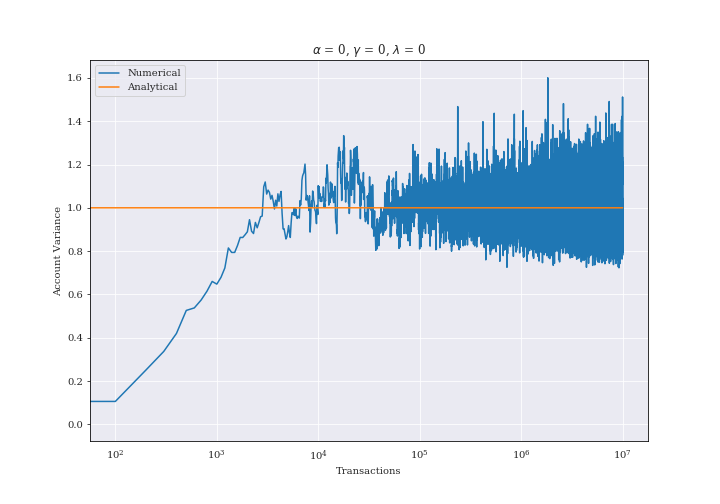
\includegraphics[scale=0.38]{parta_var.png}}
    \subfloat{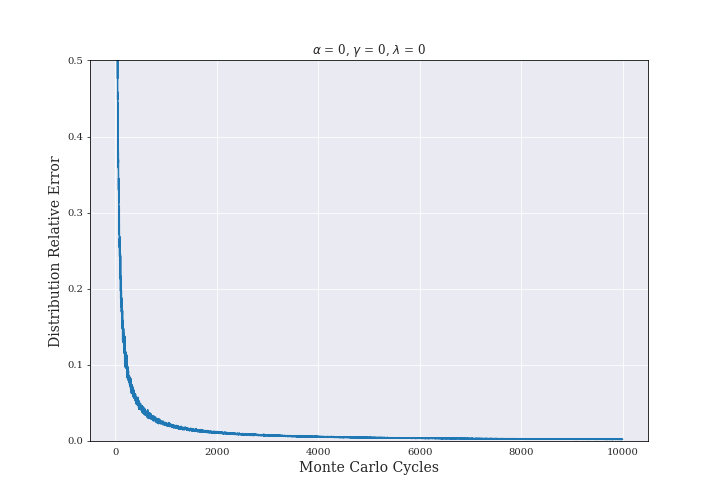
\includegraphics[scale=0.38]{parta_error.png}}\\
    \subfloat{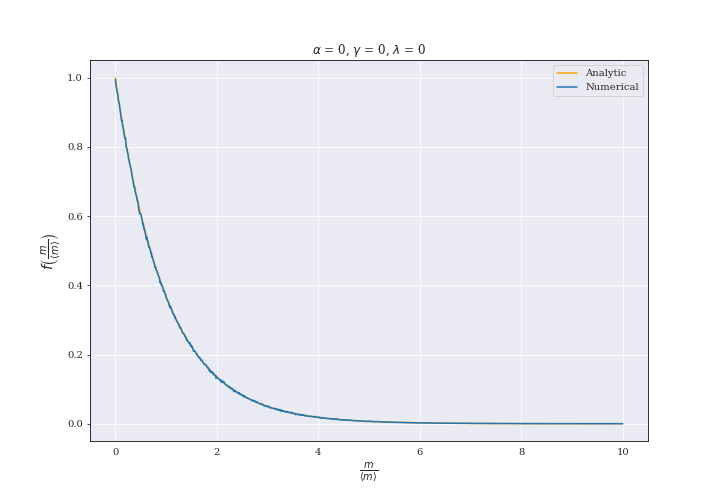
\includegraphics[scale=0.38]{parta_00_00_00.png}}
    \subfloat{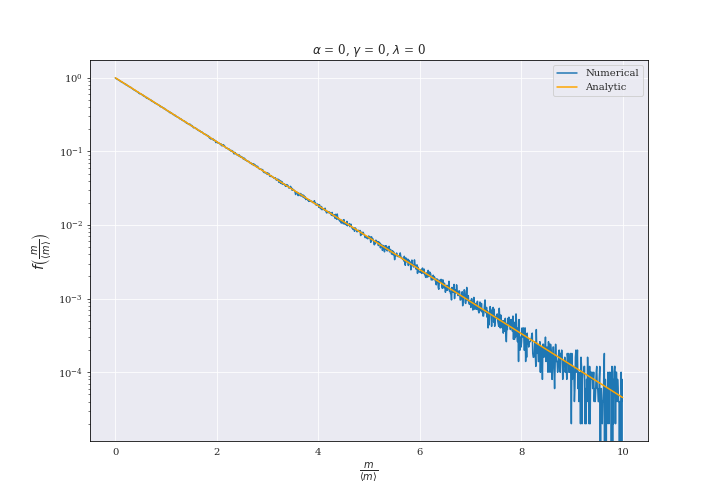
\includegraphics[scale=0.38]{partb.png}}
    \caption{The top two plots show the evolution of variance and error as well as the resulting wealth distributions. These results were obtained using $N=500$ agents and initial wealth $m_0=1000$. We see that the variance stabilizes around $10^4$ transactions and we see that the relative error between successive Monte Carlo cycles is nearly 0 at $10^4$ cycles. The distributions in the bottom two plots were obtained by performing $10^4$ transactions for each of the $10^4$ Monte Carlo cycles.}
    \label{fig1}
\end{figure*}

\begin{figure*}
        \subfloat{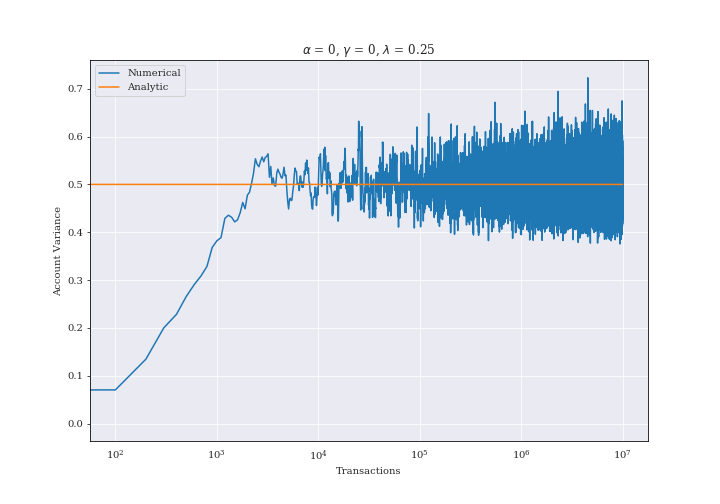
\includegraphics[scale=0.38]{partc_25_00_00_var.png}}
        \subfloat{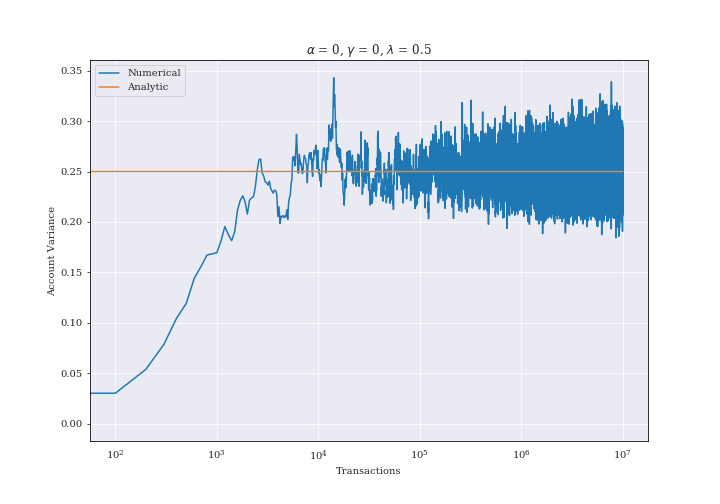
\includegraphics[scale=0.38]{partc_50_00_00_var.png}} \\
        \subfloat{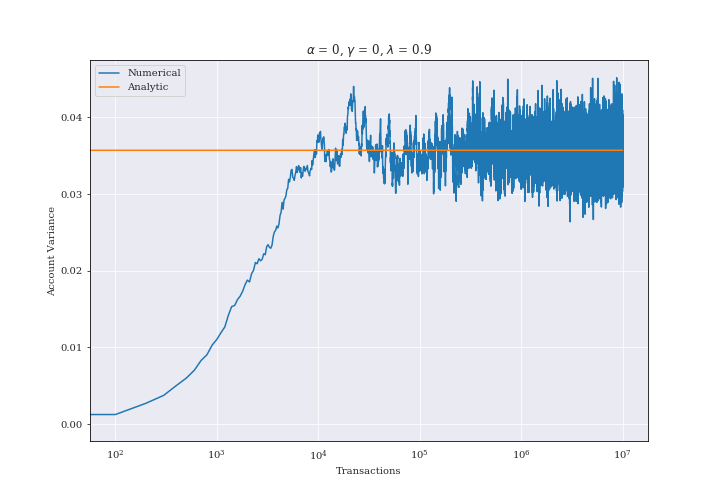
\includegraphics[scale=0.38]{partc_90_00_00_var.png}}
        \subfloat{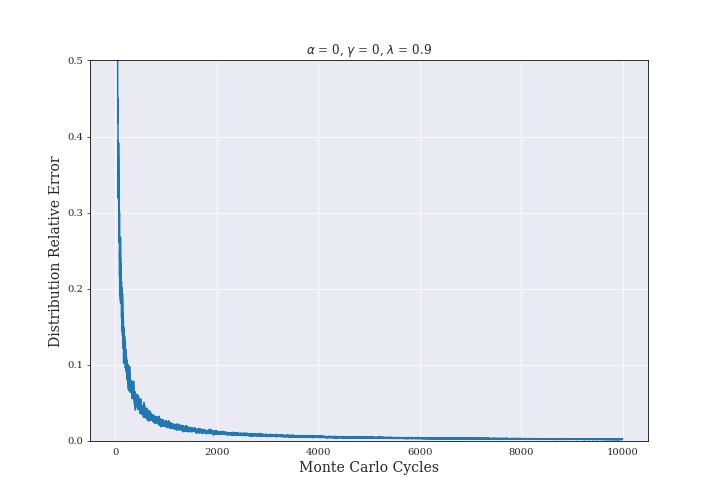
\includegraphics[scale=0.38]{partc_error.png}}
    \caption{Three plots showing the variance of account values as a function of transaction number for various values of $\lambda$. The error plot is shown only for $\lambda = 0.9$. These values were obtained using $N=500$ agents and initial wealth $m_0=1000$.}
    \label{fig2}
\end{figure*}

\begin{figure*}
        \subfloat{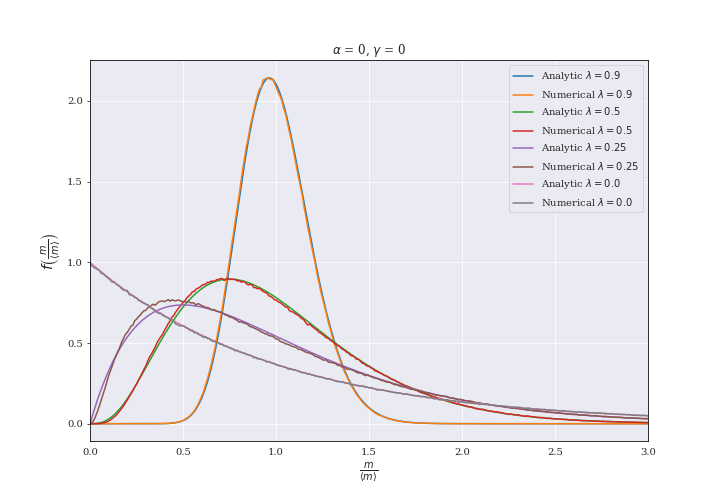
\includegraphics[scale=0.38]{partc_dist.png}}
        \subfloat{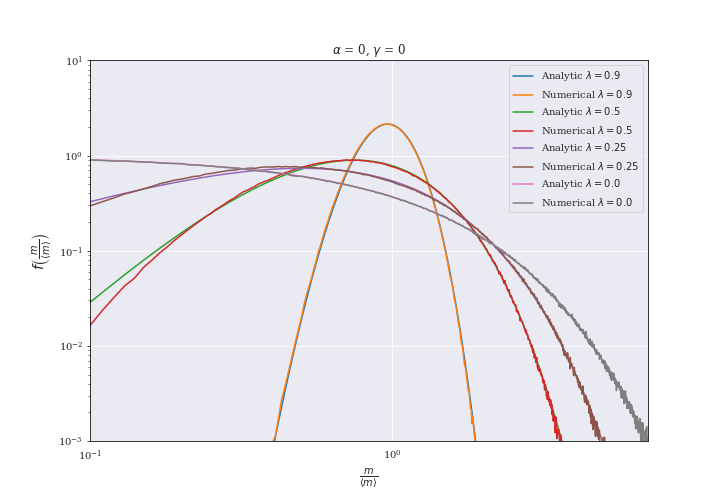
\includegraphics[scale=0.38]{partc_logdist.png}} \\
        \subfloat{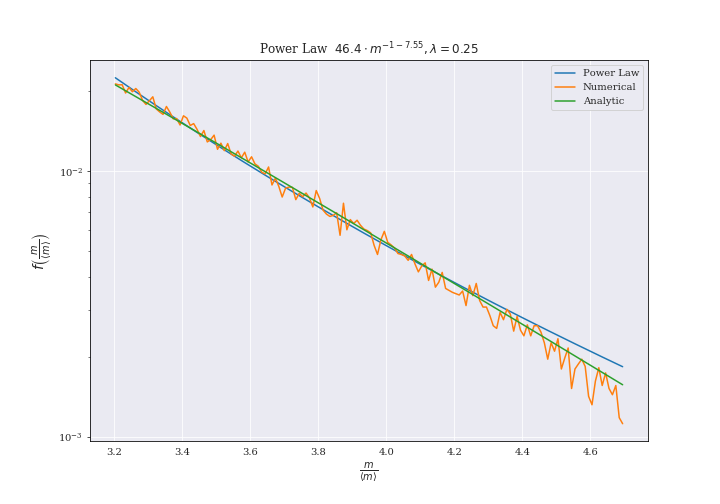
\includegraphics[scale=0.38]{partc_tail_25.png}}
        \subfloat{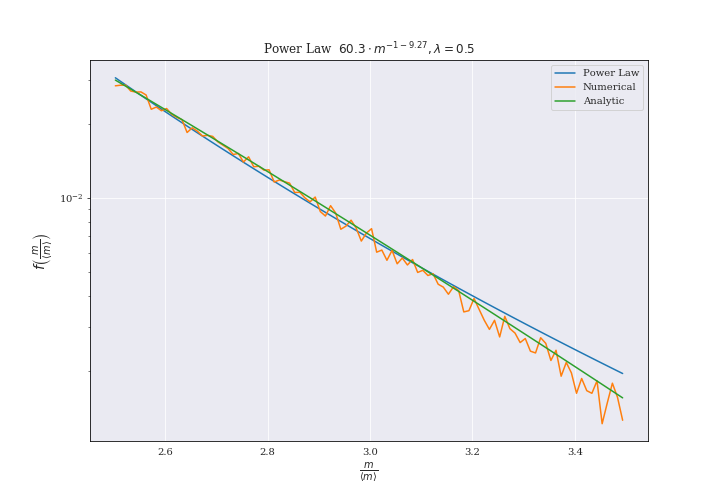
\includegraphics[scale=0.38]{partc_tail_50.png}} \\
        \subfloat{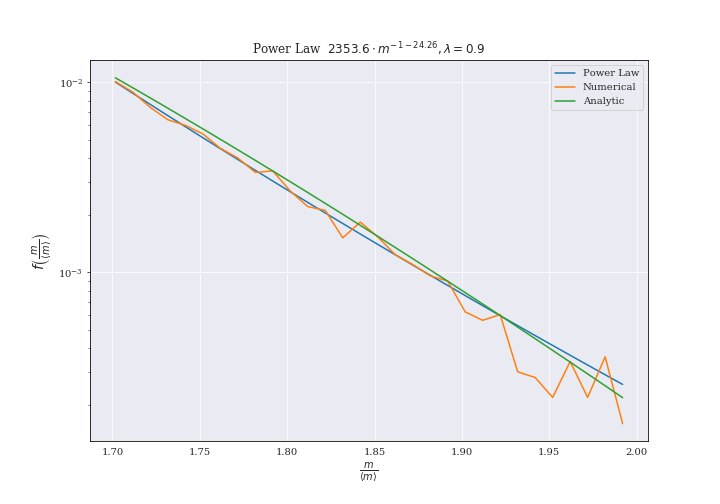
\includegraphics[scale=0.38]{partc_tail_90.png}}
    \caption{The top two plots show the resulting wealth distributions for various values of the saving parameter $\lambda$ plotted on linear and log scales. The analytical distributions are also plotted. These values were obtained using $N=500$ agents, initial wealth $m_0=1000$, $10^4$ transactions per MC cycle, and $10^4$ MC cycles. The bottom three plots show the behavior of the tail ends of the distributions shown in the top two pictures. These plots show also a power law fit of the numerical results and the analytical results.}
    \label{fig3}
\end{figure*}

\begin{figure*}
        \subfloat{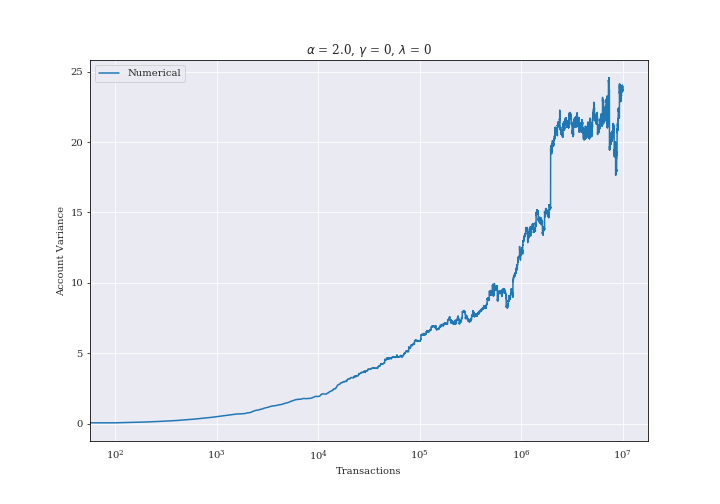
\includegraphics[scale=0.38]{partd_00_20_00_var.png}}
        \subfloat{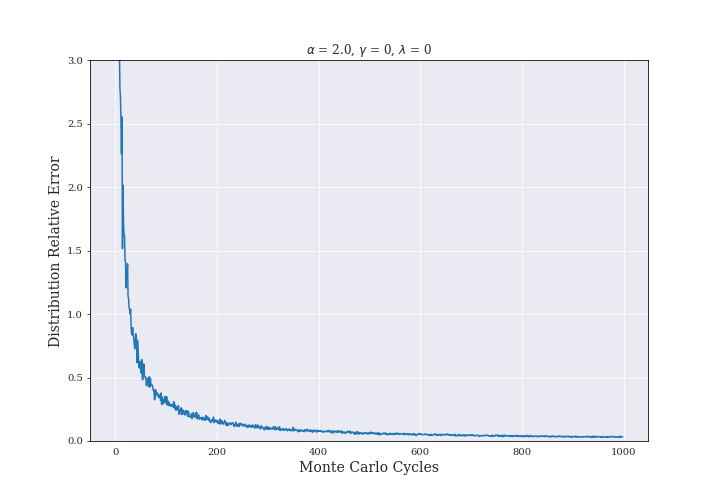
\includegraphics[scale=0.38]{partd_error.png}} \\
        \subfloat{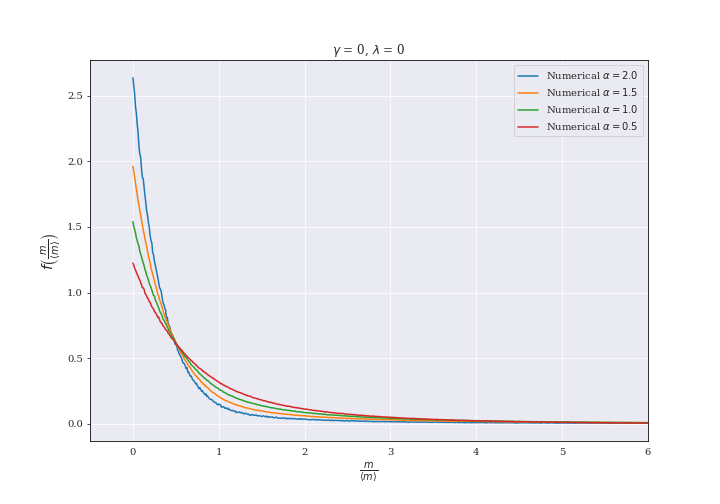
\includegraphics[scale=0.38]{partd_dist_00_00.png}}
        \subfloat{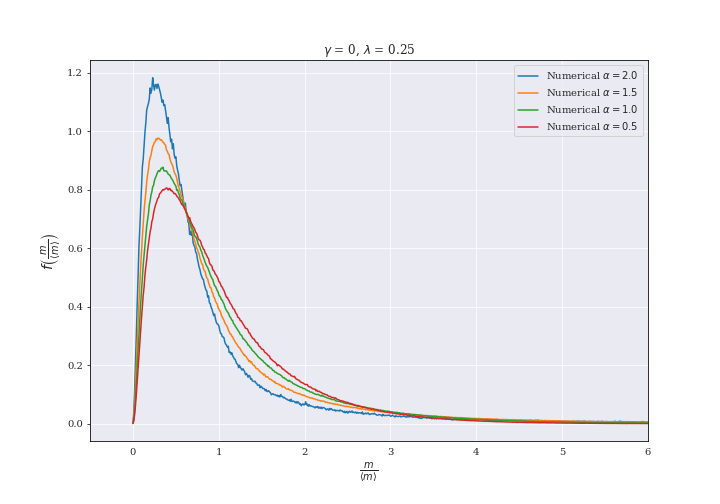
\includegraphics[scale=0.38]{partd_dist_25_00.png}}\\
        \subfloat{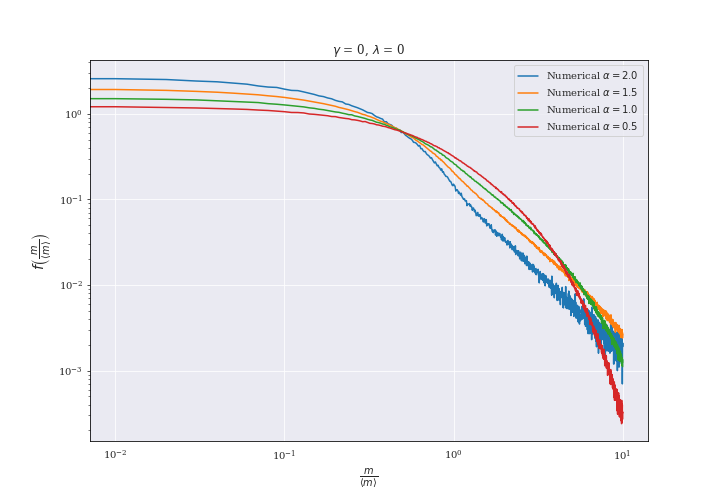
\includegraphics[scale=0.38]{partd_logdist_00_00.png}}
        \subfloat{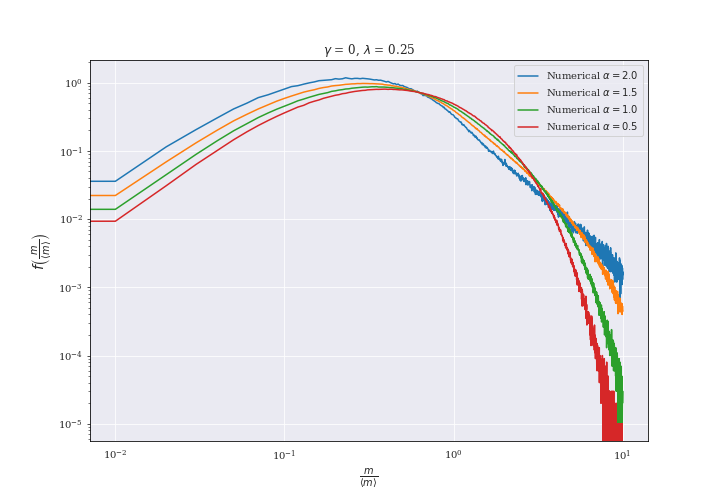
\includegraphics[scale=0.38]{partd_logdist_25_00.png}}
    \caption{The top two plots show the evolution of the variance and the difference between distributions as functions of transactions and Monte Carlo cycles. The results were obtained using $N=1000$ agents and initial wealth $m_0 = 1000$. The following four plots show the wealth distributions for systems with various strengths of wealth preference between traders ($\alpha$) both with and without saving ($\lambda$). $5\times10^6$ transactions were used for each of the $10^3$ Monte Carlo cycles.}
    \label{fig4}
\end{figure*}

\begin{figure*}
        \subfloat{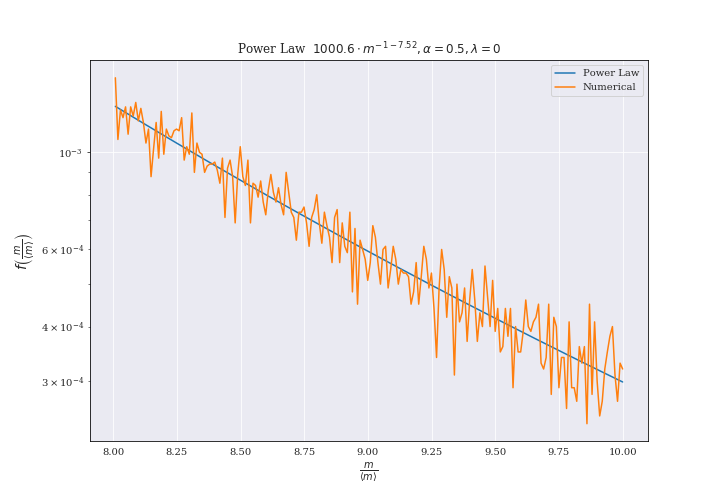
\includegraphics[scale=0.38]{partd_tail_00_05.png}}
        \subfloat{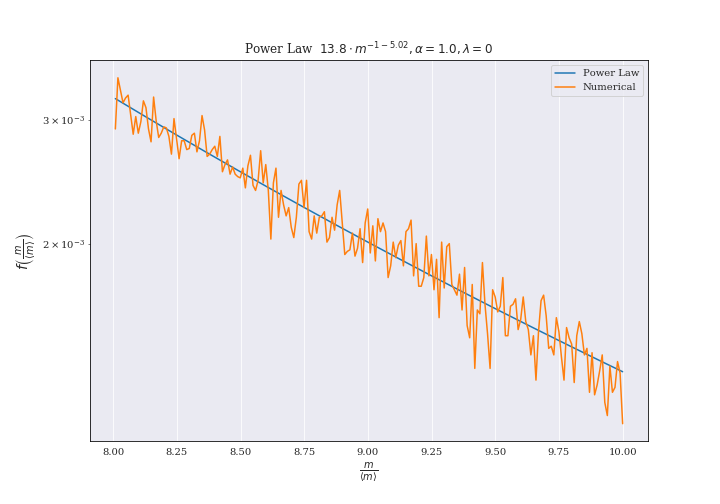
\includegraphics[scale=0.38]{partd_tail_00_10.png}} \\
        \subfloat{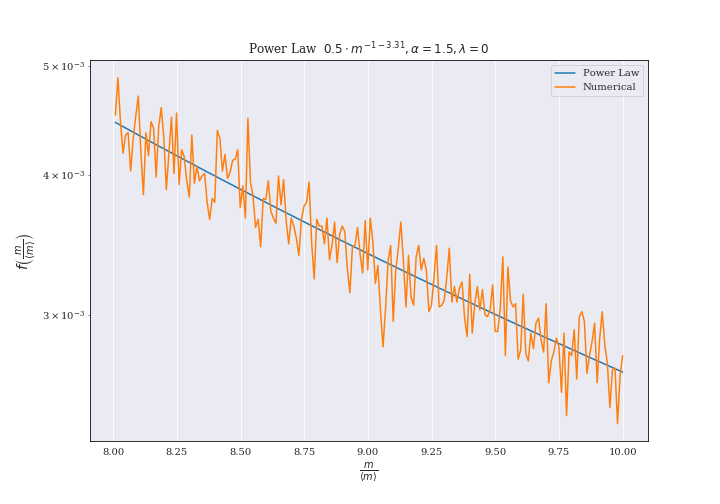
\includegraphics[scale=0.38]{partd_tail_00_15.png}}
        \subfloat{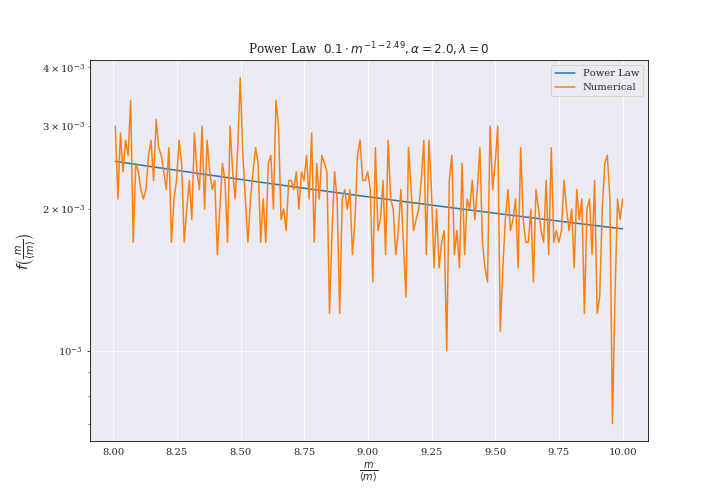
\includegraphics[scale=0.38]{partd_tail_00_20.png}}\\
    \caption{Here the tail behaviors from the distributions in the lower left plot of \ref{fig5} are shown. These results were obtained without taking saving ($\lambda$) into consideration. The resulting equations of the Power Law fits are shown above each plot.}
    \label{fig5}
\end{figure*}

\begin{figure*}
        \subfloat{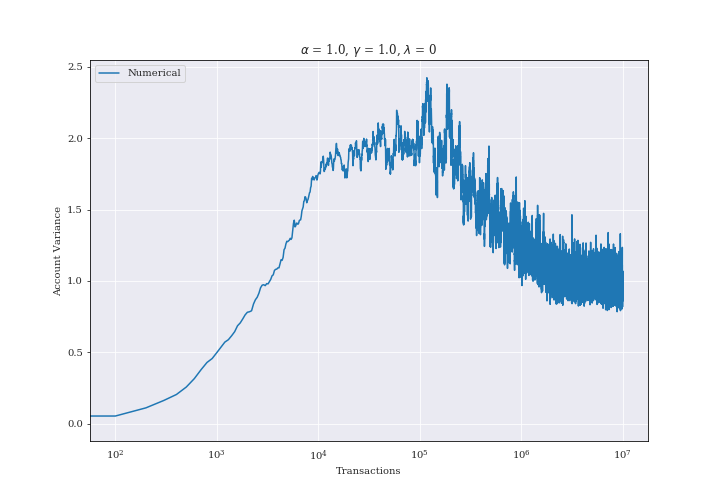
\includegraphics[scale=0.38]{parte_00_10_10_var.png}}
        \subfloat{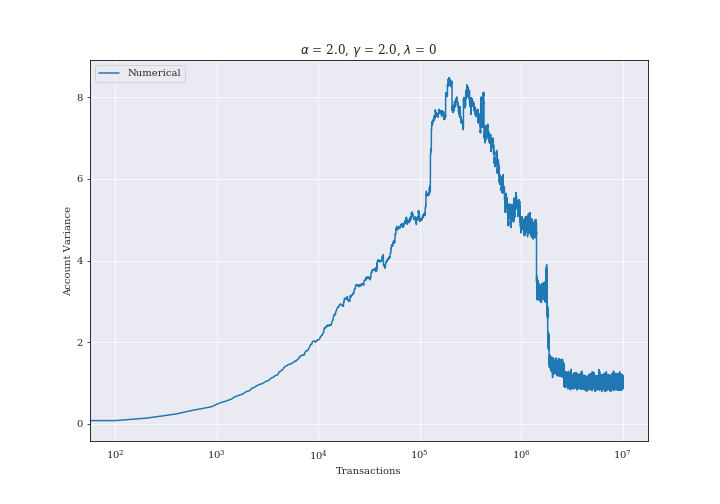
\includegraphics[scale=0.38]{parte_00_20_20_var.png}} \\
        \subfloat{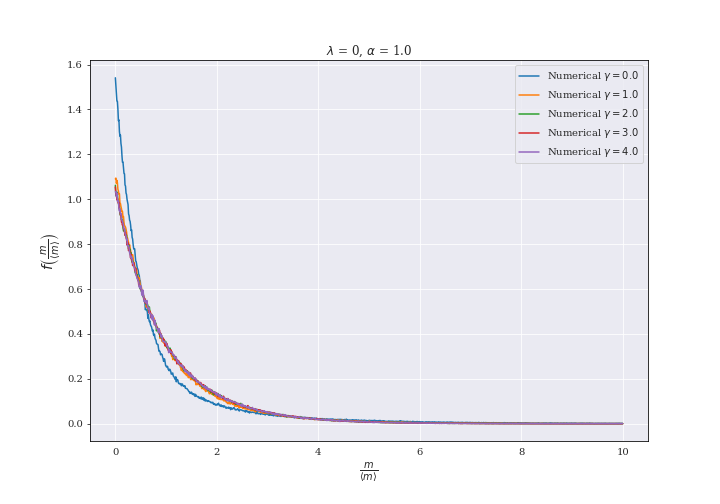
\includegraphics[scale=0.38]{parte_00_10_dist.png}}
        \subfloat{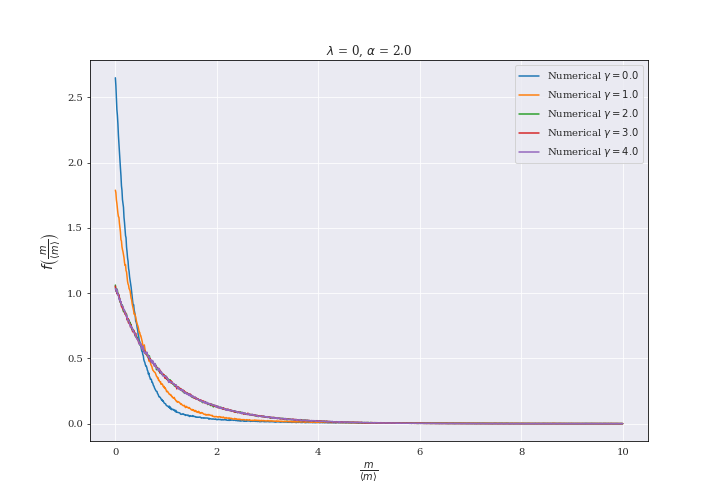
\includegraphics[scale=0.38]{parte_00_20_dist.png}}\\
        \subfloat{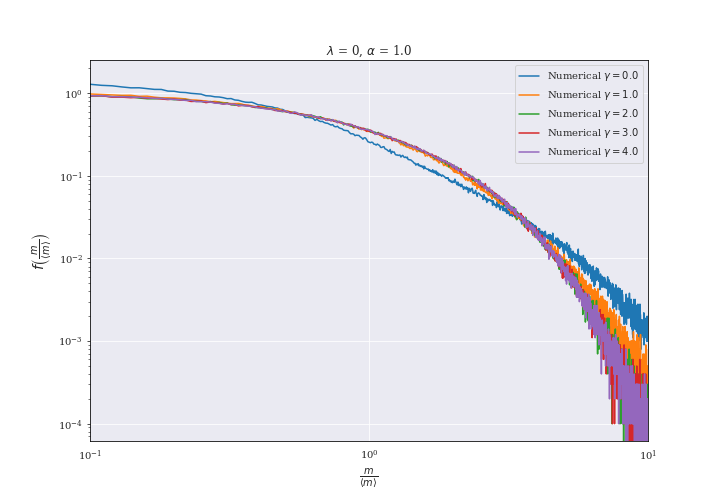
\includegraphics[scale=0.38]{parte_00_10_logdist.png}}
        \subfloat{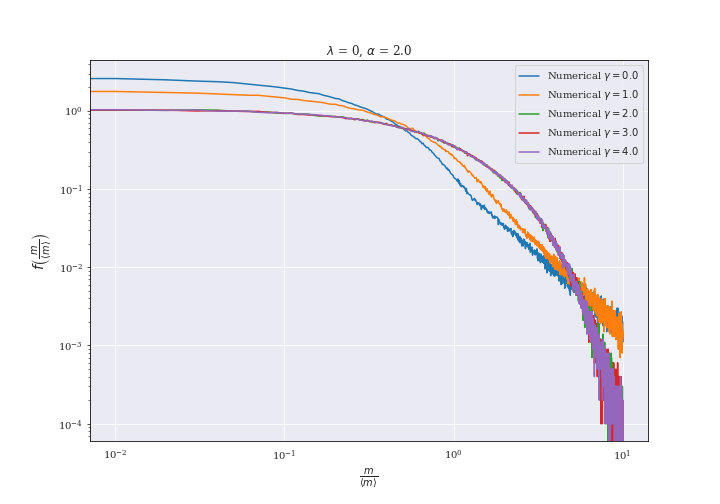
\includegraphics[scale=0.38]{parte_00_20_logdist.png}}
    \caption{The top two plots show the evolution of the variance and the difference between distributions as functions of transactions and Monte Carlo cycles. The results were obtained using $N=1000$ agents and initial wealth $m_0 = 1000$. The following four plots show the wealth distributions for systems with various strengths of wealth preference between traders ($\alpha = 1.0 or 2.0$) and various strengths of previous transaction preference ($\gamma$). $5\times10^6$ transactions were used for each of the $10^3$ Monte Carlo cycles.}
    \label{fig6}
\end{figure*}

\begin{figure*}
        \subfloat{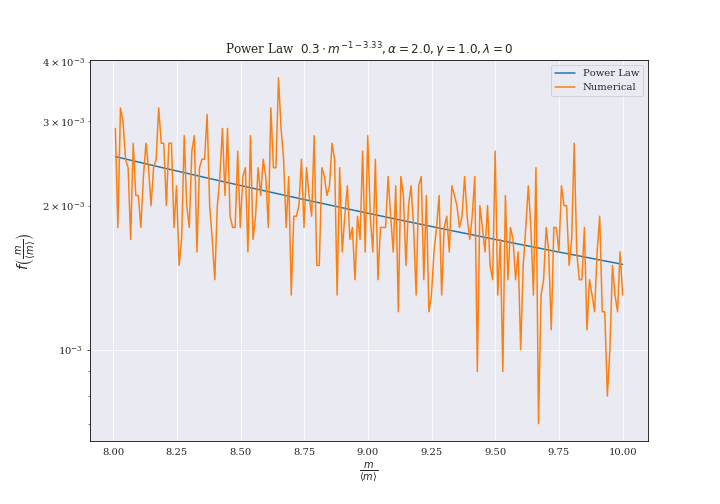
\includegraphics[scale=0.38]{parte_tail_00_20_10.png}}
        \subfloat{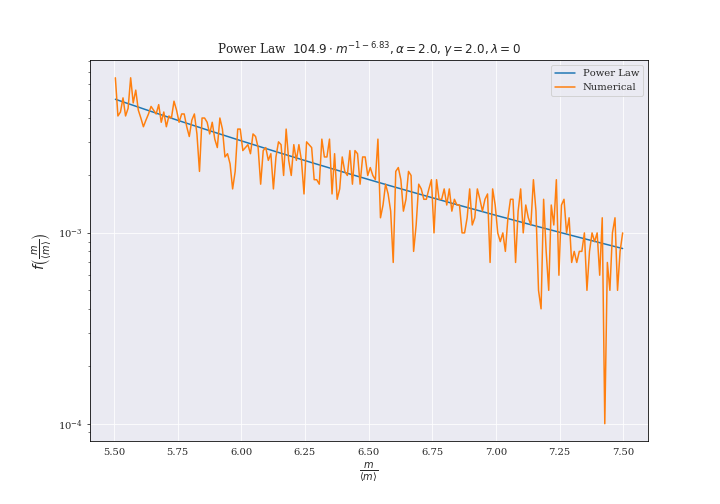
\includegraphics[scale=0.38]{parte_tail_00_20_20.png}} \\
        \subfloat{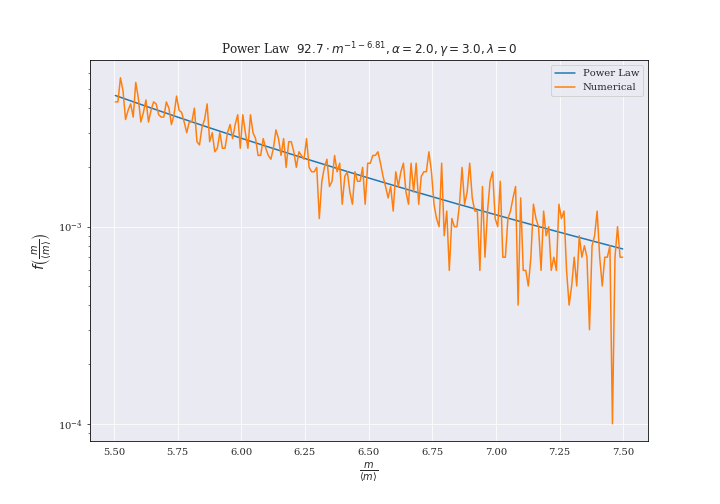
\includegraphics[scale=0.38]{parte_tail_00_20_30.png}}
        \subfloat{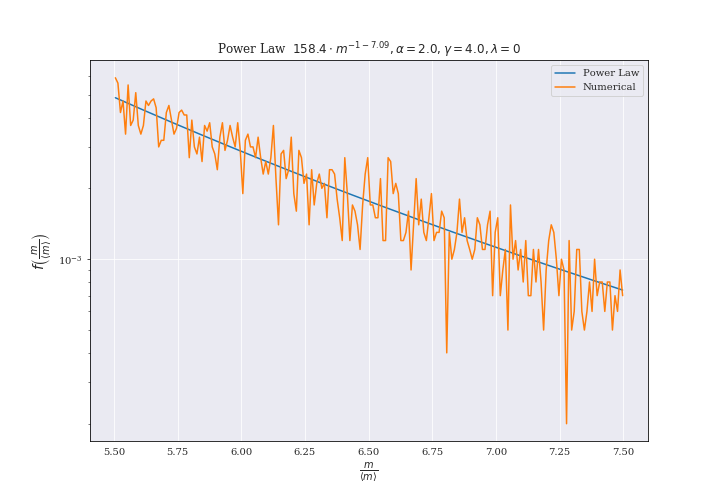
\includegraphics[scale=0.38]{parte_tail_00_20_40.png}}\\
    \caption{Here the tail behaviors from the distributions in the lower right plot of \ref{fig6} are shown. These results were obtained without taking saving ($\lambda$) into consideration and for a fixed $\alpha = 2.0$. The resulting equations of the Power Law fits are shown above each plot.}
    \label{fig7}
\end{figure*}

\begin{figure*}
        \subfloat{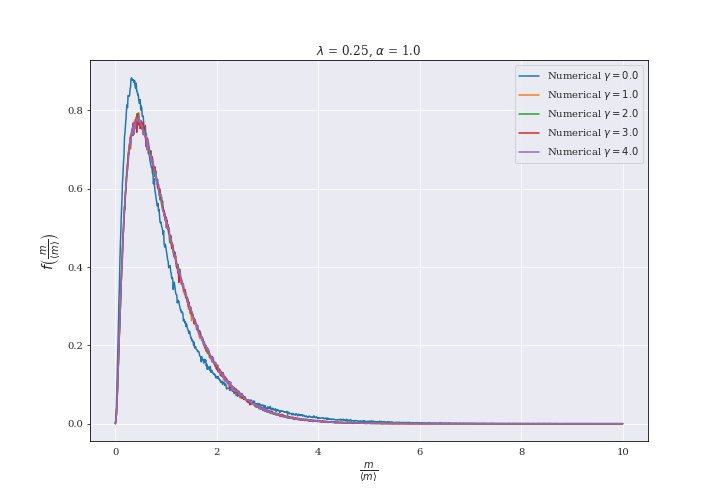
\includegraphics[scale=0.38]{parte_25_10_dist.png}}
        \subfloat{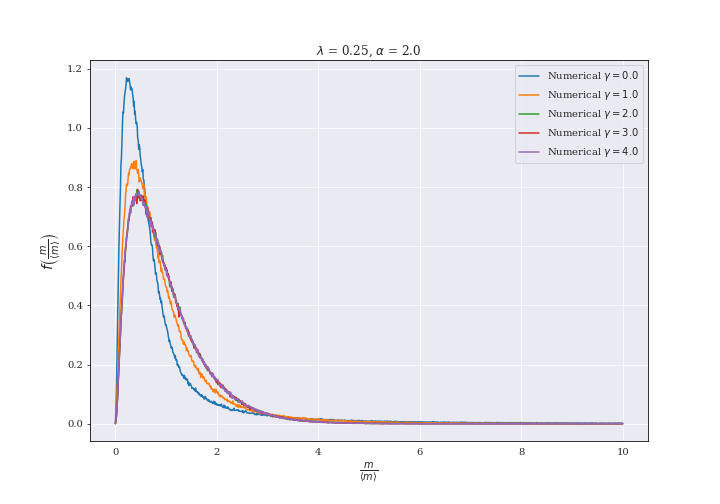
\includegraphics[scale=0.38]{parte_25_20_dist.png}} \\
        \subfloat{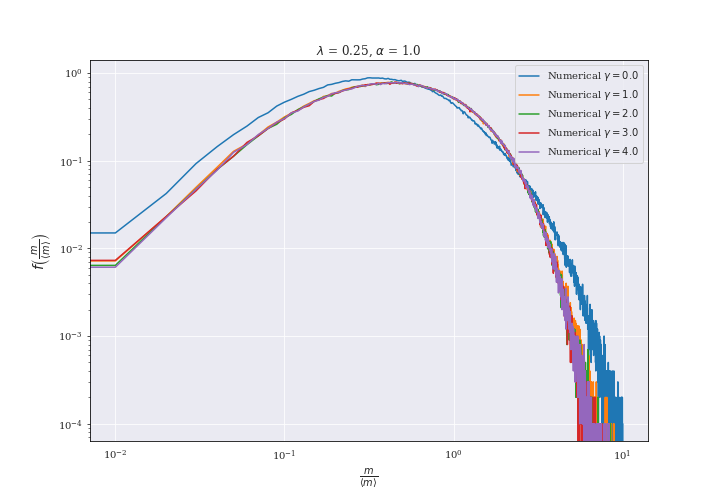
\includegraphics[scale=0.38]{parte_25_10_logdist.png}}
        \subfloat{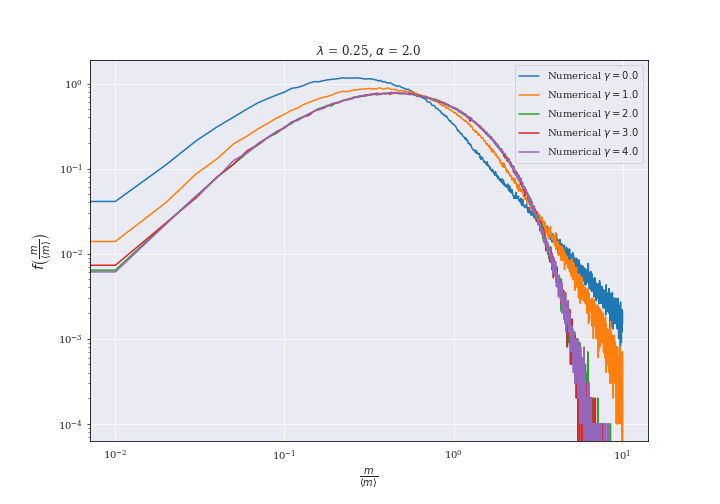
\includegraphics[scale=0.38]{parte_25_20_logdist.png}}\\
    \caption{ The following four plots show the wealth distributions for systems with various strengths of wealth preference between traders ($\alpha = 1.0 or 2.0$) and various strengths of previous transaction preference ($\gamma$) while also having a saving parameter of $\lambda = 0.25$. $5\times10^6$ transactions were used for each of the $10^3$ Monte Carlo cycles and the results were obtained using $N=1000$ agents and initial wealth $m_0 = 1000$.}
    \label{fig8}
\end{figure*}

\begin{figure*}
        \subfloat{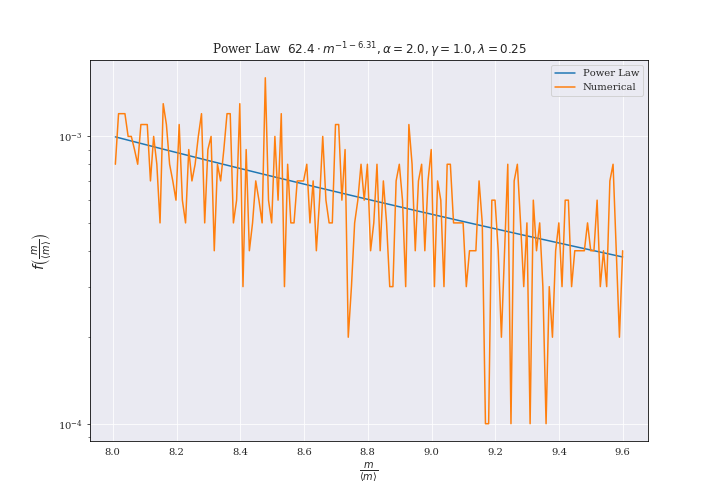
\includegraphics[scale=0.38]{parte_tail_25_20_10.png}}
        \subfloat{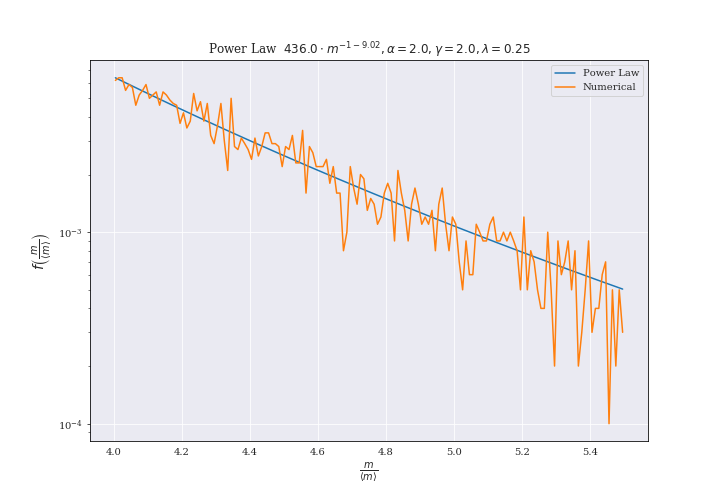
\includegraphics[scale=0.38]{parte_tail_25_20_20.png}} \\
        \subfloat{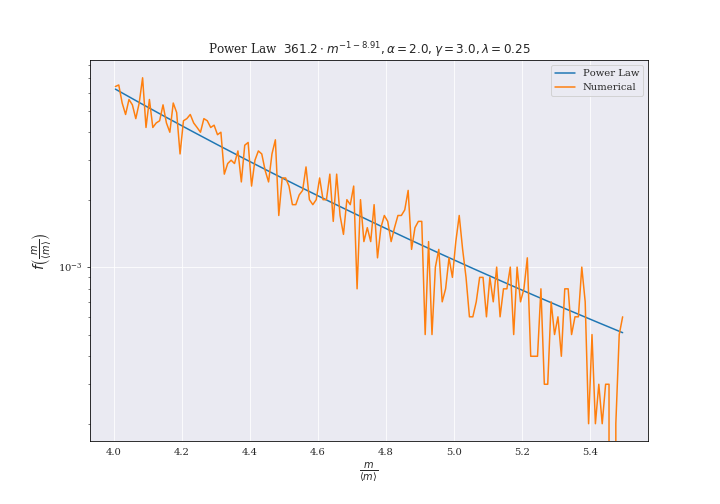
\includegraphics[scale=0.38]{parte_tail_25_20_30.png}}
        \subfloat{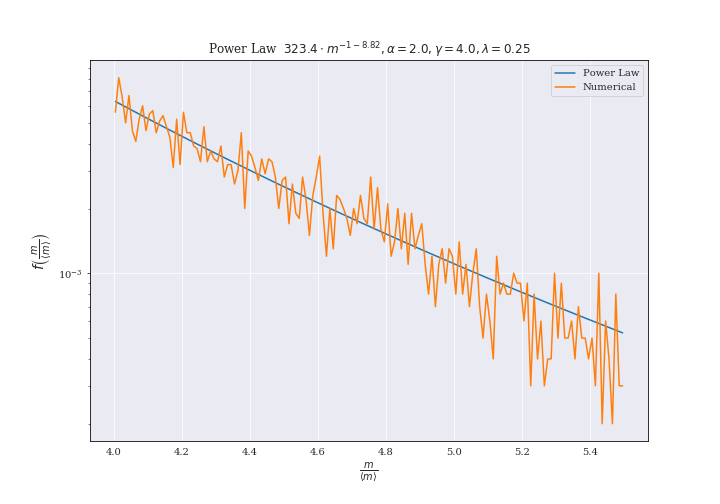
\includegraphics[scale=0.38]{parte_tail_25_20_40.png}}\\
    \caption{Here the tail behaviors from the distributions in the lower right plot of \ref{fig8} are shown. These results were obtained for a fixed saving parameter $\lambda = 0.25$ and a fixed wealth preference factor $\alpha = 2.0$. The resulting equations of the Power Law fits are shown above each plot.}
    \label{fig9}
\end{figure*}

\end{document}
